% !TEX root =  main.tex
The \mEdhoc{} \mSpec{} \cite{selander-lake-edhoc-01} claims
that \mEdhoc{} satisfies many security properties, but these are imprecisely
expressed and motivated.
%
In particular, there is no coherent adversary model.
%
Therefore, we explore in which adversary models we can prove properties and
incorporate those models into the properties themselves.
%

Next we describe our approach towards formalizing the \mEdhoc{} protocol and the
properties we verify.
%

\subsection{General Adversary Model}\label{sec:threat-model}
We verify \mEdhoc{} in the symbolic Dolev-Yao model, where
cryptographic primitives are idealized, e.g, encrypted messages can only be
decrypted with access to the key, and no hash collisions exist.
%
The adversary fully controls the
communication channel, and can interact with an unbounded number of sessions
of the protocol, dropping, injecting and modifying messages at their liking.
%

In addition to the basic Dolev-Yao model we consider three more advanced, but
yet common, adversary capabilities, namely long-term key reveal, temporary
access to long-term key and ephemeral key reveal.
%
The long-term key reveal leak a party's long-term key to the adversary.
%
This models compromise of the long-term key of a party $A$, and we denote this
type of event \mRevLTK$(A)$.
%
Temporary access to a party's long-term key provides the adversary temporary
access to the cryptographic operations of the protocol without learning the
long-term key itself.
%
This models that the adversary has temporary access to a Trusted Execution
Environment (TEE), e.g., a smart-card, in which the long-term key is stored.
%
We denote such an access to party $A$'s trusted execution environment by
\mTEE$(A)$.
%
We use this to model weak post-compromise security properties.
%
Finally, ephemeral key reveal leaks the DH half-key of a party $A$, and is
denoted \mRevEph$(A)$.
%


    \knote{Most state-of-the-art Tamarin models of real-world protocols
        (involving DH) do not
        reveal the actual session key used for the secure channel, e.g., Cremers
        et~al.~\cite{DBLP:conf/ccs/CremersFKN20}, Girol
        et~al.~\cite{DBLP:conf/uss/GirolHSJCB20}. Similarly to us, they instead
        only leak the session state (only ephemeral keys in out case).  We had
        serious problems getting Tamarin to terminate if leaking actual session
        key. Is this a common problem in Tamarin?  "All" computational models
        have session key reveal queries. CK and eCK have session state (eph-key)
        reveal queries as well.
    }
\subsection{Verified Properties}
\label{sec:desired-properties}
Our model is based on event traces and we define the
properties in terms of relations between timestamped events.
%
The model and properties are encoded for the \mTamarin{} verification tool.
%
\mTamarin{} uses an LTL-style temporal logic to reason about events and
knowledge of parties and the adversary.
%
For compactness of the presentation, we use a slightly different syntax, which
has a direct mapping to \mTamarin{}'s logic.
%

Event types are predicates over global states of the system executions.
%
Let $E$ be an event type and let $t$ be a timestamp indicating a point in a
trace.
%
Then $E^{t}$ denotes an event of type $E$ at time $t$ in that trace.
%
An event type $E$ may be associated with a sequence of parameters
$(p_i)_{i\in\mathbb{N}}$, and an event of that type at time $t$ is then
written $E^t(p_i)_{i\in\mathbb{N}}$.
%
This corresponds to \mTamarin{}'s notation for actions
$E(p_i)_{i\in\mathbb{N}}@t$.
%
In general, more than one event may have the same timestamp and hence
timestamps form a quasi order, which we denote by $t_1 \lessdot t_2$ when $t_1$
is before $t_2$ in a trace.
%
We define $\doteq$ analogously.
%
However, two events of the same type cannot have the same timestamp, so
$t_1 \doteq t_2$ implies $E^{t_1} = E^{t_2}$.
%
Other first order logic connectives and parenthesis have their standard
interpretation.
%
A special event type $\mK$ represent adversary knowledge.
%
The notation $\mK^t(p)$ denotes that the adversary knows a parameter $p$ at
time $t$.
%
Intuitively, events of type $\mK$ evaluate to true when the parameter is in
the closure of the
parameters the adversary observed from interacting with parties using the
protocol, under the operations of the Dolev-Yao message deduction rules and
the advanced adversary capabilities up until time $t$.
%

To simplify the exposition, we do not express the properties in full detail.
%
The interested reader is referred to the \mTamarin{}
model~\cite{edhocTamarinRepo}.
%

In reference to Figure~\ref{fig:edhocFramework}, an initiator $I$ considers the
protocol run to start when it sends message \mMsgone{} and considers the run
completed when sending message \mMsgthree{}.
%
We denote the first event type \mIStart{} and the second \mIComplete{}.
%
Similarly, a responder $R$ considers the run starting when receiving
\mMsgone{}, and completing when receiving \mMsgthree{}.
%
We denote the first event type \mRStart{} and the second \mRComplete{}.
%
As is customary, the properties we show are guaranteed to hold for a party when
the party completes their part of the protocol run.\\
%

%----------------------------------------------------------------------- PFS
%\subsubsection{Secrecy}
\runhead{Secrecy}
We prove a form of \emph{Perfect Forward Secrecy} (PFS).
%
Informally, PFS captures the idea that a session key remains secret even if
a long-term key leaks in the future.
%
Generalizing PFS to any information element $x$ resulting from the protocol
run, we formalize PFS with respect to the strongest adversary model we
successfully proved, as the trace predicate
%
\begin{align*}
    \mPredPfs \triangleq
    \forall I, R, x, t_2, t_3\mLogicDot
    \mK^{t_3}(x) \land (\mIComplete^{t_2}(I, R, x)\, \lor\, & \mRComplete^{t_2}(I, R, x))
    \rightarrow\\
    &(\exists t_1\mLogicDot \mRevLTK^{t_1}(I) \land t_1 \lessdot t_2)\\
    \lor&(\exists t_1\mLogicDot \mRevLTK^{t_1}(R) \land t_1 \lessdot t_2)\\
    \lor&(\exists t_1\mLogicDot \mRevEph^{t_1}(R))
    \lor(\exists t_1\mLogicDot \mRevEph^{t_1}(I)).
\end{align*}
%
\knote{The Tamarin model is logically equivalent, but not exactly the same.
    We for instance don't actually have separate "completeI" and "completeR"
    event types in the Tamarin model, but we do here to make the pictures
    prettier.
}
The first parameter of the \mIComplete{} event represents the
identity that the initiator believes plays the initiator role, i.e., itself,
and the second parameter represents the identity the initiator believes plays
the repsonder role.
%
The first and second parameter of the \mRComplete{} event are defined the same
way.
%
The meaning of remaining variables and types should be clear from previous
descriptions.
%
The essence of the definition is that an adversary only knows $x$ if they
compromised one of the
parties long-term keys before that party completed the run, or if the adversary
compromised any of the ephemeral DH half-keys at any time after a party starts
its protocol run.
%
This is depicted in Figure~\ref{fig:pfs}.
%
\begin{figure}[h!]
    \begin{center}
        \tikzset{>=latex}
        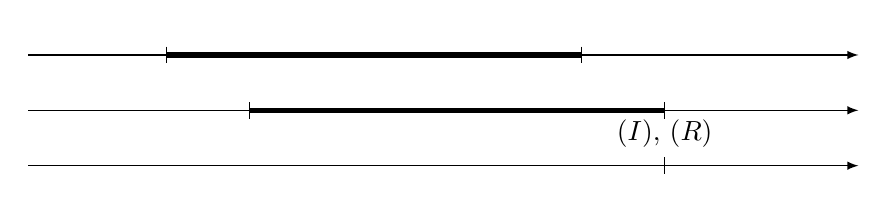
\begin{tikzpicture}
            % All units in pt
            \pgfmathsetmacro{\LOFFS}{-20} % Offset between horizontal lines
            \pgfmathsetmacro{\IS}{50}    % X-coord
            \pgfmathsetmacro{\IC}{200}    % X-coord
            \pgfmathsetmacro{\RS}{80}    % X-coord
            \pgfmathsetmacro{\RC}{230}    % X-coord
            \pgfmathsetmacro{\LTKI}{200}  % X-coord
            \pgfmathsetmacro{\LTKR}{230}  % X-coord
            % I's session ------------------------------------------------
            % Baseline
            \draw [->] (0pt,0pt) -- (300pt,0pt);
            % First event
            \draw (\IS pt,3pt) node[above] {\mIStart{}};
            \draw (\IS pt,3pt) -- (\IS pt,-3pt);
            % Second event
            \draw (\IC pt,3pt) node[above] {\mIComplete{}};
            \draw (\IC pt,3pt) -- (\IC pt,-3pt);
            % Thick session span line
            \draw [line width=2pt] (\IS pt,0pt) -- (\IC pt,0pt);
            % R's session ------------------------------------------------
            % Baseline
            \draw [->] (0pt,\LOFFS + 0pt) -- (300pt,\LOFFS + 0pt);
            % First event
            \draw (\RS pt,\LOFFS + 3pt) node[above] {\mRStart{}};
            \draw (\RS pt,\LOFFS + 3pt) -- (\RS pt,\LOFFS - 3pt);
            % Second event
            \draw (\RC pt,\LOFFS + 3pt) node[above] {\mRComplete{}};
            \draw (\RC pt,\LOFFS + 3pt) -- (\RC pt,\LOFFS - 3pt);
            % Thick session span line
            \draw [line width=2pt] (\RS pt,\LOFFS + 0pt) -- (\RC pt,\LOFFS + 0pt);
            % LTKRev(I,R)  -----------------------------------------------
            % Baseline
            \draw [->] (0pt,2*\LOFFS + 0pt) -- (300pt,2*\LOFFS + 0pt);
            % Attack events
            \draw (\LTKR pt,2*\LOFFS + 3pt) node[above] {\mRevLTK$(I)$, \mRevLTK$(R)$};
            \draw (\LTKR pt,2*\LOFFS + 3pt) -- (\LTKR pt,2*\LOFFS - 3pt);
        \end{tikzpicture}
        \caption{Perfect Forward Secrecy: the earliest the adversary can use its
                 advanced capabilities while secrecy is still maintained.
                 Ephemeral DH half-keys can never be revealed.}
        \label{fig:pfs}
    \end{center}
\end{figure}\\

%-------------------------------------------------------------------- InjAgree
%\subsubsection{Authentication}
\runhead{Authentication}
\label{sec:authenticationDef}
We prove two different flavors of authentication, the first being classical
injective agreement following Lowe~\cite{DBLP:conf/csfw/Lowe97a}, and the second
being an implicit agreement property.
%
Informally, \emph{injective agreement} guarantees to an initiator $I$
running with some responder that if, whenever $I$ completed the run and
believes the responder is $R$,
then $R$ has been engaged in the protocol in the opposite role,
and the run of $I$ corresponds to a unique run of $R$.
%
In addition, the property guarantees to $I$ that the two parties agree on a set
$S$ of parameters associated with the run, in particular the set includes the
session key material $k$.
%
However, we will treat $k$ separately for clarity.
%
On completion, $I$ knows that $R$ has access to the session key material.
%
The corresponding property for $R$ is defined analogously.
%
%This is no longer true: We model this slightly differently.
%%
%Our formulation for guaranteeing injective agreement to $I$ with $R$, enforces
%that for any session key material $k$, there can be at most one run of $I$
%involving it, and this run must map to at least one run of $R$ involving $k$.
%%
%Injective agreement for $R$ with $I$ is formulated as the dual of this.
%%
%Our formulation uniquely guarantees one run of the initiator involving $k$,
%but allows us to have potentially multiple runs of $R$ involving $k$, and vice
%versa.
%%
%However, because we prove injective agreement for both $I$ and $R$, this
%becomes equivalent to the Lowe formulation, and guarantees a unique map.
%%

Traditionally, the event types used to describe injective agreement are called
\emph{Running} and \emph{Commit}, but to harmonize the presentation of
authentication and secrecy, we refer to these events as \mIStart{} and
\mIComplete{} respectively for the initiator, and \mRStart{} and \mRComplete{}
for the responder.
%
More formally, for the initiator role we define injective agreement by the
trace predicate
\begin{align*}
    \mPredInjI& \triangleq
    \forall I, R, k, S, t_2\mLogicDot \mIComplete^{t_2}(I, R, k, S)
    \rightarrow\\
    &(\exists t_1\mLogicDot \mRStart^{t_1}(R, k, S) \land t_1 \lessdot t_2)
    \land\ (\forall I' R' t_1' \mLogicDot \mIComplete^{t_1'}(I' , R', k, S)
        \rightarrow t_1' \doteq t_1) \\
    &\lor(\exists t_1\mLogicDot \mRevLTK^{t_1}(R) \land t_1 \lessdot t_2).
\end{align*}
%
Figure~\ref{fig:injAgree} shows when the adversary at the earliest can use
advanced capabilities such that \mPredInjI{} still holds.
%
Ephemeral DH half-keys can be revealed as soon as they are created.
%
The initiator's long-term key can be revealed before any of the parties start
their runs.
%
For the responder role we define
\begin{align*}
    \mPredInjR& \triangleq\
    \forall I, R, k, S, t_2\mLogicDot \mRComplete^{t_2}(I, R, k, S)
    \rightarrow\\
    &(\exists t_1\mLogicDot \mIStart^{t_1}(I, R, k, S) \land t_1 \lessdot t_2)
    \land (\forall I' R' t_1' \mLogicDot \mRComplete^{t_1'}(I' , R', k, S)
        \rightarrow t_1' \doteq t_1)\\
    &\lor(\exists t_1\mLogicDot \mRevLTK^{t_1}(I) \land t_1 \lessdot t_2).
\end{align*}
%
Figure~\ref{fig:injAgree} depicts when the adversary at the earliest can use
advanced capabilities.
%
Ephemeral DH half-keys can be revealed as soon as they are created.
%
The responder's long-term key can be revealed before any of the parties start
their runs.
%
\begin{figure}[h!]
    \begin{center}
        \tikzset{>=latex}
        \begin{tikzpicture}
            % All units in pt
            \pgfmathsetmacro{\LOFFS}{-20} % Offset between horizontal lines
            \pgfmathsetmacro{\IS}{80}     % X-coord
            \pgfmathsetmacro{\IC}{200}    % X-coord
            \pgfmathsetmacro{\RS}{120}    % X-coord
            \pgfmathsetmacro{\RC}{230}    % X-coord
            \pgfmathsetmacro{\LTKI}{200}  % X-coord
            \pgfmathsetmacro{\LTKR}{230}  % X-coord
            \draw (-10 pt,10pt) node [above] {\mPredInjI};
            % I's session ------------------------------------------------
            % Baseline
            \draw [->] (0pt,0pt) -- (300pt,0pt);
            % First event
            \draw (\IS pt,3pt) node[above] {\mIStart{}};
            \draw (\IS pt,3pt) -- (\IS pt,-3pt);
            % Second event
            \draw (\IC pt,3pt) node[above] {\mIComplete{}};
            \draw (\IC pt,3pt) -- (\IC pt,-3pt);
            % Thick session span line
            \draw [line width=2pt] (\IS pt,0pt) -- (\IC pt,0pt);
            % R's session ------------------------------------------------
            % Baseline
            \draw [->] (0pt,\LOFFS + 0pt) -- (300pt,\LOFFS + 0pt);
            % First event
            \draw (\RS pt,\LOFFS + 3pt) node[above] {\mRStart{}};
            \draw (\RS pt,\LOFFS + 3pt) -- (\RS pt,\LOFFS - 3pt);
            % Second event
            \draw (\RC pt,\LOFFS + 3pt) node[above] {\mRComplete{}};
            \draw (\RC pt,\LOFFS + 3pt) -- (\RC pt,\LOFFS - 3pt);
            % Thick session span line
            \draw [line width=2pt] (\RS pt,\LOFFS + 0pt) -- (\RC pt,\LOFFS + 0pt);
            % LTKRev(I,R)  -----------------------------------------------
            % Baseline
            \draw [->] (0pt,2*\LOFFS + 0pt) -- (300pt,2*\LOFFS + 0pt);
            % Attack events
            \draw (\IC pt,2*\LOFFS + 3pt) node[above] {\mRevLTK$(R)$};
            \draw (\IC pt,2*\LOFFS + 3pt) -- (\IC pt,2*\LOFFS - 3pt);
            \draw (\IS - 50 pt,2*\LOFFS + 3pt) node[above] {\mRevLTK$(I)$};
            \draw (\IS - 50 pt,2*\LOFFS + 3pt) -- (\IS - 50 pt,2*\LOFFS - 3pt);
            \draw (\IS pt,2*\LOFFS + 3pt) node[above] {\mRevEph$(I)$};
            \draw (\IS pt,2*\LOFFS + 3pt) -- (\IS pt,2*\LOFFS - 3pt);
            \draw (\RS pt,2*\LOFFS + 3pt) node[above] {\mRevEph$(R)$};
            \draw (\RS pt,2*\LOFFS + 3pt) -- (\RS pt,2*\LOFFS - 3pt);
            % InjAgree for R =============================================
            \pgfmathsetmacro{\IS}{80}     % X-coord
            \pgfmathsetmacro{\IC}{200}    % X-coord
            \pgfmathsetmacro{\RS}{120}    % X-coord
            \pgfmathsetmacro{\RC}{230}    % X-coord
            \pgfmathsetmacro{\LTKI}{200}  % X-coord
            \pgfmathsetmacro{\LTKR}{230}  % X-coord
            \draw (-10 pt,4*\LOFFS+6pt) node [above] {\mPredInjR};
            % I's session ------------------------------------------------
            % Baseline
            \draw [->] (0pt,4*\LOFFS + 0pt) -- (300pt,4*\LOFFS + 0pt);
            % First event
            \draw (\IS pt,4*\LOFFS + 3pt) node[above] {\mIStart{}};
            \draw (\IS pt,4*\LOFFS + 3pt) -- (\IS pt,4*\LOFFS + -3pt);
            % Second event
            \draw (\IC pt,4*\LOFFS + 3pt) node[above] {\mIComplete{}};
            \draw (\IC pt,4*\LOFFS + 3pt) -- (\IC pt,4*\LOFFS + -3pt);
            % Thick session span line
            \draw [line width=2pt] (\IS pt,4*\LOFFS + 0pt) -- (\IC pt,4*\LOFFS + 0pt);
            % R's session ------------------------------------------------
            % Baseline
            \draw [->] (0pt,5*\LOFFS + 0pt) -- (300pt,5*\LOFFS + 0pt);
            % First event
            \draw (\RS pt,5*\LOFFS + 3pt) node[above] {\mRStart{}};
            \draw (\RS pt,5*\LOFFS + 3pt) -- (\RS pt,5*\LOFFS - 3pt);
            % Second event
            \draw (\RC pt,5*\LOFFS + 3pt) node[above] {\mRComplete{}};
            \draw (\RC pt,5*\LOFFS + 3pt) -- (\RC pt,5*\LOFFS - 3pt);
            % Thick session span line
            \draw [line width=2pt] (\RS pt,5*\LOFFS + 0pt) -- (\RC pt,5*\LOFFS + 0pt);
            % LTKRev(I,R)  -----------------------------------------------
            % Baseline
            \draw [->] (0pt,6*\LOFFS + 0pt) -- (300pt,6*\LOFFS + 0pt);
            % Attack events
            \draw (\RC pt,6*\LOFFS + 3pt) node[above] {\mRevLTK$(I)$};
            \draw (\RC pt,6*\LOFFS + 3pt) -- (\RC pt,6*\LOFFS - 3pt);
            \draw (\IS - 50 pt,6*\LOFFS + 3pt) node[above] {\mRevLTK$(R)$};
            \draw (\IS - 50 pt,6*\LOFFS + 3pt) -- (\IS - 50 pt,6*\LOFFS - 3pt);
            \draw (\IS pt,6*\LOFFS + 3pt) node[above] {\mRevEph$(I)$};
            \draw (\IS pt,6*\LOFFS + 3pt) -- (\IS pt,6*\LOFFS - 3pt);
            \draw (\RS pt,6*\LOFFS + 3pt) node[above] {\mRevEph$(R)$};
            \draw (\RS pt,6*\LOFFS + 3pt) -- (\RS pt,6*\LOFFS - 3pt);
        \end{tikzpicture}
        \caption{Injective agreement guarantee: the earliest the
        adversary can use its advanced capabilities such that the properties
        are still proven to be maintained.}
        \label{fig:injAgree}
    \end{center}
\end{figure}
%

%------------------------------------------------------------- Implicit auth
Not all \mEdhoc{} methods have the injective agreement property, so we show
for all methods a form of \emph{implicit agreement} on all the parameters
mentioned above.
%
We take inspiration from the computational model definitions of implicit
authentication proposed by Guilhem~et~al.~\cite{DBLP:conf/csfw/GuilhemFW20} to
modify the classical injective agreement into an implicit property.
%
An important difference between our definition and theirs, is that they focus on
authenticating a key and related identities, whereas we extend the more general
concept of agreeing on a set of parameters, deriving from the idea of injective
agreement~\cite{DBLP:conf/csfw/Lowe97a}.
%
We use the term \emph{implicit} in this context to refer to that a party
accepts any other party who knows the session key material as the
authenticated party, and that party (if honest) will also agree on the
parameters computed by the protocol.
%
The intuition behind our definition is that a party $A$, being either initiator
or responder, may complete a protocol
run resulting in a set of parameters $S$, one of which is a session key $k$,
and $A$ then believes these parameters can be agreed with another party $B$.
%
When completing, $A$ is then guaranteed that $B$ has been or is
engaged in exactly one protocol run with $A$ in the opposite role, and that $B$
has or will be able to agree on $S$.
%
This allows $A$ to conclude that if the last message reaches $B$, then
$A$ and $B$ have agreed on $S$.
%
In contrast to injective agreement, this property is symmetric with respect to
the roles.
%
In particular, because the guarantee only reasons about completed and
hypothetically completed protocol runs, it can reason about parameters that the
responder learns only after receiving the last message.
%
In contrast to almost full explicit key authentication defined by
Guilhem~et~al.~\cite{DBLP:conf/csfw/GuilhemFW20}, our definition does not
require key confirmation, so our definition is indeed closer to their implicit
authentication.
%
Also here we split the property into one guarantee for the initiator $I$ and
one for $R$, but only show the definition for $I$.
%
The definition for $I$ is
\begin{align*}
    \mPredImpI& \triangleq
    \forall I, R, k, S, t_1\mLogicDot \mIComplete^{t_1}(I, R, k, S)
    \rightarrow\\
      &(\forall I', R', S', t_2\mLogicDot \mRComplete^{t_2}(I', R', k, S') \rightarrow
             (I=I' \land R=R' \land S=S'))\\
      \land &(\forall I', R', S', t_1'\mLogicDot
        (\mIComplete^{t_1'}(I', R', k, S') \rightarrow t_1' \doteq t_1
        )\\
    &\lor(\exists t_0\mLogicDot \mRevLTK^{t_0}(R) \land t_0 \lessdot t_1)
    \lor(\exists t_0\mLogicDot \mRevEph^{t_0}(R))
    \lor(\exists t_0\mLogicDot \mRevEph^{t_0}(I)).
\end{align*}
%
Figure~\ref{fig:impAgreeI} depicts when the adversary at the earliest can use
advanced capabilities.
%
Ephemeral DH half-keys can never be revealed, and the responder's long-term key
can be revealed once the initiator completes its run.
%
The initiator's long-term key can be revealed before any of the parties start
their runs.
%
\begin{figure}[h!]
    \begin{center}
        \tikzset{>=latex}
        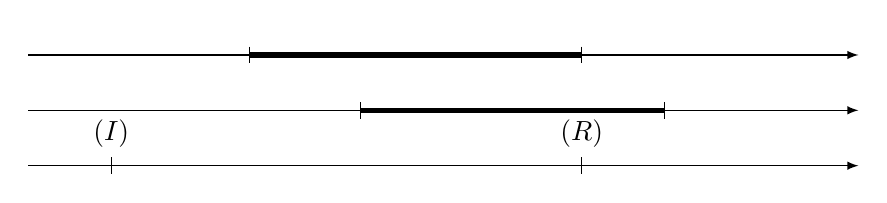
\begin{tikzpicture}
            % All units in pt
            \pgfmathsetmacro{\LOFFS}{-20} % Offset between horizontal lines
            \pgfmathsetmacro{\IS}{80}     % X-coord
            \pgfmathsetmacro{\IC}{200}    % X-coord
            \pgfmathsetmacro{\RS}{120}    % X-coord
            \pgfmathsetmacro{\RC}{230}    % X-coord
            \pgfmathsetmacro{\LTKI}{200}  % X-coord
            \pgfmathsetmacro{\LTKR}{230}  % X-coord
            % I's session ------------------------------------------------
            % Baseline
            \draw [->] (0pt,0pt) -- (300pt,0pt);
            % First event
            \draw (\IS pt,3pt) node[above] {\mIStart{}};
            \draw (\IS pt,3pt) -- (\IS pt,-3pt);
            % Second event
            \draw (\IC pt,3pt) node[above] {\mIComplete{}};
            \draw (\IC pt,3pt) -- (\IC pt,-3pt);
            % Thick session span line
            \draw [line width=2pt] (\IS pt,0pt) -- (\IC pt,0pt);
            % R's session ------------------------------------------------
            % Baseline
            \draw [->] (0pt,\LOFFS + 0pt) -- (300pt,\LOFFS + 0pt);
            % First event
            \draw (\RS pt,\LOFFS + 3pt) node[above] {\mRStart{}};
            \draw (\RS pt,\LOFFS + 3pt) -- (\RS pt,\LOFFS - 3pt);
            % Second event
            \draw (\RC pt,\LOFFS + 3pt) node[above] {\mRComplete{}};
            \draw (\RC pt,\LOFFS + 3pt) -- (\RC pt,\LOFFS - 3pt);
            % Thick session span line
            \draw [line width=2pt] (\RS pt,\LOFFS + 0pt) -- (\RC pt,\LOFFS + 0pt);
            % LTKRev(I,R)  -----------------------------------------------
            % Baseline
            \draw [->] (0pt,2*\LOFFS + 0pt) -- (300pt,2*\LOFFS + 0pt);
            % Attack events
            \draw (\IC pt,2*\LOFFS + 3pt) node[above] {\mRevLTK$(R)$};
            \draw (\IC pt,2*\LOFFS + 3pt) -- (\IC pt,2*\LOFFS - 3pt);
            \draw (\IS - 50 pt,2*\LOFFS + 3pt) node[above] {\mRevLTK$(I)$};
            \draw (\IS - 50 pt,2*\LOFFS + 3pt) -- (\IS - 50 pt,2*\LOFFS - 3pt);
        \end{tikzpicture}
        \caption{Implicit agreement guarantee for $I$: the earliest the
        adversary can use its advanced capabilities. Ephemeral keys can never be
        revealed.}
        \label{fig:impAgreeI}
    \end{center}
\end{figure}
%
The responder's guarantee is an defined analogously, letting initiator and
repsonder events swap places, and letting long-term key reveal events swap
places.\\
%

%------------------------------------------------------- Agreed parameters
\runhead{Agreed Parameters}
%\subsubsection{Agreed Parameters}
The initiator $I$ gets injective and implicit agreement guarantees on the
following set $S_\mEdhoc$ of parameters:
\begin{itemize}
    \item responder identity,
    \item the roles played by itself and its peer,
    \item session key material (which varies depending on \mEdhoc{} method),
    \item context identifiers \mCi{} and \mCr{}, and
    \item cipher suites \mSuites{}.
\end{itemize}
%
Because of \mEdhoc{} aiming to provide identity protection for $I$, there is no
injective agreement guarantee for $I$ that $R$ agrees on the initiator identity.
%
For the same reason, there is neither any such guarantee for $I$ with respect to
the \mGiy{} part of the session key material when $I$ uses a \mStat{}-based
method.
%
There is, however, an implicit agreement guarantee for $I$ that $R$ agrees on
$I$'s identity and the full session key material.
%
Since $R$ completes after $I$, $R$ can get injective agreement guarantees on
more parameters, namely the initator's identity and the full session key
material for all methods.\\
%

%------------------------------------------------------- Implied properties
\runhead{Subsumed Properties}
%\subsubsection{Subsumed Properties}
Given the secrecy and agreement properties and parameter set $S_\mEdhoc$ defined
above, other properties can be indirectly concluded to hold.
%
Protocols where a party does not get confirmation on that their peer knows the
session key material are known to be at risk to
\emph{Key-Compromise Impersonation (KCI)}
attacks~\cite{DBLP:conf/ima/Blake-WilsonJM97}.
%
Attacks in this class allows an adversary in possession of a party's secret
long-term key to coerce that party to complete a
protocol run believing it authenticated a certain peer, but where that peer did
not engage in a run.
%
Because both our notions of agreement above ensure agreement on identities,
roles and session key material, all methods passing verification of those also
have resistance to KCI attacks.
%

If a party can be coerced into believing it completed a run with a peer $A$, but
where the session key material is actuality shared with a party $B$, the used
protocol is vulnerable to an \emph{Unknown Key-Share (UKS)}
attack~\cite{DBLP:conf/ima/Blake-WilsonJM97}.
%
For the same reason as for KCI, a protocol passing verification of our agreement
properties is also resistant to UKS attacks.
%

Our agreement properties also capture \emph{entity authentication}.
%


%Achieving injective agreement on the roles and the
%identities of the parties in those roles implies \emph{entity authentication}.
%
%In addition, achieving injective agreement on the session key material implies
%\emph{session key material authentication}.
%

%
%We say that \mEdhoc{} in method $m$ satisfies \emph{explicit authentication} for
%the initiator $I$ with a responder $R$, if injective agreement holds for $I$
%with $R$ on the session key $sk$, when running method $m$.
%%
%The corresponding definition for the responder is analogous.
%%
%If both parties obtain explicit authentication we refer to it as mutual explicit
%authentication (or simply explicit authentication).
%%
%A party $A$ is guaranteed explicit authentication when both parties have
%agreement on fresh session key material, each others identities and roles
%(and other parameters), when $A$ completes the protocol run.
%%
%Because they have (cryptographically justified) agreement on each others
%identities, it follows that explicit authentication implies entity
%authentication.
%%
%As we discuss later, it turned out that explicit authentication does not hold for all
%\mEdhoc{} methods, in which cases we prove \emph{implicit authentication}.

%Computational models often rely on implicit session key authentication
%(see, for example, the definition of SK-security in the Canetti-Krawczyk
%model~\cite{DBLP:conf/crypto/CanettiK02}).
%%
%Although symbolic models predominantly rely on correspondence properties
%in the style of Lowe~\cite{DBLP:conf/csfw/Lowe97a}, there are examples where
%implicit session key authentication has been used.
%%
%For example, Schmidt~et~al.~\cite{DBLP:conf/csfw/SchmidtMCB12} use a
%symbolized version of an extended Canetti-Krawzcyk model.

%%
%We say that a protocol satisfies \emph{implicit authentication} if the
%initiator and responder agree on the session key only after both parties
%successfully completes the protocol.
%%
%That is, authentication is implicit, as the
%initiator receives no confirmation that the responder has computed the same session key.
%%
%More precisely, we adapt the definition of~\cite{DBLP:journals/iacr/GuilhemFW19}
%to the symbolic model, and we prove that if an initiator $I$ and a responder $R$
%complete the protocol deriving the same session key, then $I$ believes they are
%talking to $R$ and vice versa.
%%

\knote{I propose we remove all discussions about what the spec claims (except
    that it is imprecise and unclear. There is simply too many loose statements
there that does not coherently add up to treat all those claims. Discussing some of them
here does not seem to make sense to me.}
%\mEdhoc{} claims to support mutual authentication with consistency, aliveness
%and peer awareness (see Section~\ref{sec:claimedProperties}).
%%
%These claims appear to have been imported from \mSigma{}~\cite{sigma}, using the
%inheritance argument, because all three appear there as well.
%%
%The definition of consistency~\cite{sigma} is very close in intent to the
%definition we use for implicit authentication, except that it is posed in a
%computational setting.
%%
%We therefore consider them equal in terms of intent for the purpose of this
%paper.
%%
%Aliveness is, according to \mSigma{}~\cite{sigma}, guaranteed to a party $A$ if
%after running the protocol with $B$, $A$ knows that $B$ was alive during
%the execution, e.g., by verifying that $B$ signed a challenge.
%%
%For \mEdhoc{} this means that if we can prove mutual injective agreement, i.e.,
%explicit authentication, on \mGxy{}, then mutual aliveness follows.
%%
%Peer awareness is informally defined in~\cite{sigma} as the guarantee
%that if $A$ completes a protocol run with $B$, then not only does $A$
%know that $B$ is alive, but also that $B$ has initiated a corresponding session
%with $A$.
%\\

%\runhead{Perfect Forward Secrecy (PFS)}
%%\subsubsection{Perfect Forward Secrecy} 
%Perfect forward
%secrecy holds if, for any run in which the initiator and the responder
%agree on a session key $sk$ and any of their long-term keys are revealed after
%the run is complete, the attacker does still not learn $sk$.

 
%\subsubsection{Key-Compromise Impersonation} (KCI) This property takes the perspective of one
%of the endpoints of the protocol, say Alice running a session with Bob. A
%protocol is secure under KCI if Alice can still establish a secure session with
%Bob, even though Alice's keys are compromised at any time, and Bob's key
%material is not leaked until the end of the session.
%
% 
%\subsubsection{Post-Compromise Security} (PCS) A protocol that has
%\emph{post-compromise security} (following definitions in~\cite{cohn2016post})
%is capable of establishing a secure session even after one of the parties has
%been compromised. Cohn-Cordon et al.~\cite{cohn2016post} presents two notions of
%PCS, namely weak and strong PCS: here we focus on the latter.
%%
%A protocol guarantees \emph{weak PCS} if secrecy of any session key $sk$ holds
%between the initiator and the responder, even if the run of the protocol that
%established $sk$ happens after a \emph{limited compromise}, where the key
%material is not leaked, but the attacker is capable of impersonating both
%parties (i.e. has the ability to perform all cryptographic operations using the
%initiator's and responder's long term keys, but has not access to the long term
%keys).

 
%With the first rule we allow the protocol to decrypt the message \mT{m} if the encryption has matching key \mT{k}, authenticated data \mT{ad}, and uses the same algorithm \mT{al}.
%
%The second rule allows the attacker to decrypt the message \mT{m} with the key
%\mT{k} and without the authenticated data \mT{ad}, and hence skip the check.

%The built-in theories for XOR and Diffie-Hellman are a fair bit more complex
%than authenticated encryption, hence we refer to the original
%papers~\cite{DBLP:conf/csfw/DreierHRS18,DBLP:conf/csfw/SchmidtMCB12}
%for a full reference.
%

 
%\subsubsection{Syntactic Sugar} In the following presentation we use some syntactic
%sugar, namely
%the use of let bindings (\mT{let ... in}), which are series of
%definitions of patterns which are substituted in the rest of the rule. %Another
%prominent feature is the use of tuples (\mT{<t1, ..., tn>}) which are a
%built-in concept in \mTamarin.

%---------------------------------------------------------------------------
\subsection{\mTamarin{}}
\label{sec:tamarin}
 
We chose \mTamarin{} to model and verify \mEdhoc{} in the symbolic model.
%
\mTamarin{} is an interactive verification tool based on multi-set rewrite rules
with event annotations based on action facts, which allow the user to check
 LTL-style formulas on these models as mentioned above.
%
Multi-set rewrite rules with action facts look like $ l \ifarrow[e] r $,
where $l$ and $r$ are multi-sets of facts, and $e$ is a multi-set of action facts.
Facts are $n$-ary predicates over a term algebra, which defines a set of function
symbols $\mathcal F$, variables $\mathcal V$ and names $\mathcal N$. \mTamarin{}
checks equality of these terms under an equational theory $E$. For example,
one can write $ dec(enc(x,y),y) =_E x $
to denote that symmetric decryption reverses the encryption operation under this theory.
The equational theory $E$ is fixed per model, and hence we omit the subscript.
\mTamarin{} supports let-bindings and tuples as syntactic sugar to simplify model
definitions. \\

%\runhead{Semantics and Built-ins}
%%\subsubsection{Semantics and Built-ins} \phantom{} 
%\mTamarin{} states
%$S$, $S'$ are multisets of facts, and a semantic transition of the form $S \semarrow[E] S'$
%occurs if there is a rule $l \ifarrow[e] r$ and a substitution $\sigma$ such
%that $S \supseteq \sigma(l)$ and $S' = S \setminus \sigma(l) \uplus \sigma(r)$
%and $E = \sigma(e)$.
%
%There are a few more details, such as persistent facts which are denoted by a $!$
%and are never removed from the state.
%%
%The sorts fresh (denoted by $\sim$) and public (denoted by $\$$) denote fresh
%constants and public values known to the attacker respectively, and are both
%sub-sorts of a base sort.
%%
%Finally, \mTamarin{} has some built-in predicates ($\mIn,
%\mOut$ to represent input and output of messages with the attacker,
%and
%$\mFr$ to denote a fresh constant created in the current rule, among
%others), rules and equations that represent the attacker's knowledge
%and standard equational theories in the symbolic model,
%which we present later.

%\anote{This can go, I make a shorter note later:\\
%{Notational conventions} In the remainder of this section we present
%\mTamarin{} code as it appears in the models that we verify, in the style of
%literate programming.  Whenever possible we match the style of the protocol
%diagrams in Section~\ref{sec:edhoc} and the naming convention of the \mEdhoc{}
%\mSpec~\cite{selander-lake-edhoc-01}, so that each element of the model is
%traceable to the standard.  There are a few exceptions to this, most notably
%some variable names that we introduce for the sake of the \mTamarin{} model and are
%not present in the original \mSpec{}, which will appear in \mT{camelCase}, and
%the syntax for Diffie-Hellman exponentiation which is specific to \mTamarin{}.
%We also use \mT{xx} to name the ephemeral key for the initiator (resp. \mT{yy}
%for the responder) as to avoid confusion with \mTamarin's builtin variable
%names \mT{x} and \mT{y}.}

\runhead{Protocol Rules and Equations}
%\subsubsection{Protocol Rules and Equations}
\mTamarin{} allows users to define new function symbols and equational theories.
These user defined objects are then translated by \mTamarin{} into rewrite
rules, which are added to the set of considered rules during verification.
For example, in our model we have a symbol to denote authenticated encryption, for which \mTamarin{} produces the following rule:
%
\begin{lstlisting}
[!KU(k), !KU(m), !KU(ad), !KU(al)] --> [!KU(aeadEncrypt(k, m, ad, al))]
\end{lstlisting}
%
to denote that if the attacker knows a key \mT{k}, a message \mT{m}, the
authenticated data \mT{ad}, and an algorithm \mT{al}, then they can construct
the encryption using these parameters, and thus get to know the message
\lstinline{aeadEncrypt(k, m, ad, al)}.

In our model we make use of
the built-in theories of exclusive-or and DH operations, as in~\cite{DBLP:conf/csfw/DreierHRS18,DBLP:conf/csfw/SchmidtMCB12}.
%
%The XOR theory introduces the symbol \mT{XOR}, plus the necessary equational theory including associativity, commutativity, and inverse.
%
%The Diffie-Hellman theory introduces exponentiation \mT{g^y} and product of exponents \mT{x * y} as built-in symbols in the language, plus the necessary equational theory of associativity, commutativity, distributivity of exponentiation with product, and inverse.
For \mAead{} operations, we add the following equations:
\begin{lstlisting}
aeadDecrypt(k, aeadEncrypt(k, m, ad, al), ad, al) = m
decrypt(k, aeadEncrypt(k, m, ad, al), al) = m
\end{lstlisting}
Both the above equations govern decryption. The first rule checks to see if the authenticated data is as expected, while the second rule skips this check.


 
%-------------------------------------------------------------------------- sub
\subsection{Modeling \mEdhoc{}}
\label{sec:modeling} 
In this section we detail the modeling choices that we have made for this formal
verification effort.
%
We model the five different methods of \mEdhoc{} from a single specification
using the M4 macro language to derive all valid combinations: \mPskPsk,
\mSigSig, \mSigStat, \mStatSig{} and \mStatStat.
%
Whenever possible we adhere with the variable names present in the \mSpec{} and
in Section~\ref{sec:edhoc}.
%
There are a few exceptions: we use \mT{camelCase} for names introduced in the modeling, and we use \mT{xx} and
\mT{yy} for the ephemeral keys, to avoid name clashes.
%
To keep the presentation brief, we only present the \mStatSig{} mode, as it
shows both asymmetric authentication methods at the same time.
%
%More details on the \mPskPsk{} method and 
All \mTamarin{} models can be
found at~\cite{edhocTamarinRepo}.
\\
%\anote{Fix: give a dropbox link instead of the repo}
%

%\subsubsection{General Setup}
\runhead{General Setup}
The following rules express the registering of the long term keys for the
\mSig{}- and \mStat{}-based methods, respectively.
%
\begin{lstlisting}
rule registerLTK_SIG:
 [Fr(~ltk)] --[ UniqLTK($A, ~ltk) ]->
  [!LTK_SIG($A, ~ltk), !PK_SIG($A, pk(~ltk)), Out(<!<$A, pk(~ltk)>!>)]
rule registerLTK_STAT:
 [Fr(~ltk)] --[ UniqLTK($A, 'g'^~ltk) ]->
  [!LTK_STAT($A, ~ltk), !PK_STAT($A, 'g'^~ltk), Out(<!<$A, 'g'^~ltk>!>)]
\end{lstlisting}
%
The rules \mT{registerLTK_SIG} and \mT{registerLTK_STAT} register a public key
(for signing and static DH exchange, respectively) which is tied to the
identity of an agent \mT{A}.
%
A similar rule \mT{registerLTK_PSK} registers pre-shared symmetric keys for
pairs of agents.
%
The event \mT{UniqLTK} together with a corresponding restriction models the fact that
the long-term key is unique for each agent.
% or pair of agents, as enforced by the following restriction:
% \begin{lstlisting}
% restriction uniqLTKs:
%     "All id k1 k2 #i #j. (UniqLTK(id, k1)@i & UniqLTK(id, k2)@j) ==> k1 = k2"
% \end{lstlisting}
This models that there is an external mechanism ensuring that the
long term keys are bound to the correct identity, e.g., a certificate authority.
%
It also models that the attacker cannot register new public keys for an
existing identity.
%

We also introduce rules to give the attacker access to
long-term keys and session keys.
%and the cryptographic interface of the device.
%
\begin{lstlisting}
rule revealLTK_SIG: [!LTK_SIG($A, ~ltk)] --[LTKRev($A)]-> [Out(~ltk)]
rule revealLTK_STAT: [!LTK_STAT($A, ~ltk)] --[LTKRev($A)]-> [Out(~ltk)]
rule revealSessionKeyI: [CommitI(tid, u, v, sk)] --[SKRev(sk)]-> [Out(sk)]
rule revealSessionKeyR: [CommitR(tid, u, v, sk)] --[SKRev(sk)]-> [Out(sk)]
\end{lstlisting}
%rule forge_SIG: [!LTK_SIG($A, ~ltk), In(xx)] --[TEE($A)]-> [Out(sign(xx, ~ltk))]
%rule exp_STAT: [!LTK_STAT($A, ~ltk), In('g'^x)] --[TEE($A)]-> [Out(('g'^x)^~ltk)]
%
These are used to model long-term key compromise and session key secrecy.
\\
%These rules allow to check Perfect Forward Secrecy, Key Compromise Impersonation
%and (weak) Post Compromise Security as defined in Section~\ref{sec:desired-properties},
%by giving the attacker the ability to access to long term and session keys, or
%to the cryptographic interface, at the appropriate time.

%\subsubsection{Modeling Choices}
\runhead{Modeling Choices}
We model each method of the protocol with four rules: \mT{I1}, \mT{R2}, \mT{I3}
and \mT{R4} (with the current method suffixed to the rule name).
%
Each of these represent one step of the protocol as run by the initiator \mT{I}
and the responder \mT{R}.
%
The rules can be traced back to the diagrams of
Figure~\ref{fig:edhocsigstat} and Figure~\ref{fig:edhocstatsig}.
%

Our model differs slightly from the \mSpec{}.
%
In particular, for convenience we divide the \mMethod{} element into two
elements, representing the method for the initiator and the responder without
reducing the attacker potential.
%
To make the model manageable we omit the connection identifiers \mCi{} and
\mCr{}, and represent the selected cipher suite by the public variable
\mT{\$cSUITES0}, known to the attacker.
%
We plan to introduce the connection identifiers in our ongoing verification
effort.
%
The way we model the selected cipher suite implies that our model does not
capture the possibility for the responder to reject the initiator's offer. 
%

%We model the XOR encryption of \mT{CIPHERTEXT_2} with the key \mT{K_2e} as to
%allow recovering of part of the key for known plaintext.
%
%Hence \mT{CIPHERTEXT_2} is not a direct XOR ``encryption'' in the model, but
%rather a tuple where each field is XORed with a half-key expansion (\mT{K_2e_1}
%and \mT{K_2e_2}).
We model the XOR encryption of \mT{CIPHERTEXT_2} with the key \mT{K_2e} using
\mTamarin{}'s built in theory for XOR, and allow each term of the encrypted
element to be attacked individually.
%
That is, we first expand \mT{K_2e} to as many key-stream terms as there are
terms in the plaintext tuple using the \mHkdfExpand{} function in a counter-mode
of operation.
%
We then XOR each term in the plaintext with its own key-stream term.
%
This models the \mSpec{} closer than if we would have XORed \mT{K_2e}, as a
single term, onto the plaintext tuple.
%
The XOR encryption can be seen in on line 16-19 in the listing of
\mT{R2_STAT_SIG} below.
%
\begin{lstlisting}
rule R2_STAT_SIG:
  let
    data_2 = <'g'^~yy>
    m1 = <'STAT', 'SIG', $cSUITE0, gx>
    TH_2 = h(<$cHash0, m1, data_2>)
    prk_2e = hkdfExtract('emptyStr', gx^~yy)
    prk_3e2m = prk_2e
    K_2m = hkdfExpand(<$cAEAD0, TH_2, 'K_2m'>, prk_3e2m)
    protected2 = $V // ID_CRED_V
    CRED_V = pkV
    extAad2 = <TH_2, CRED_V>
    assocData2 = <protected2, extAad2>
    MAC_2 = aeadEncrypt('emptyStr', K_2m, assocData2, $cAEAD0)
    authV = sign(<assocData2, MAC_2>, ~ltk)
    plainText2 = <$V, authV>
    K_2e = hkdfExpand(<$cAEAD0, TH_2, 'K_2e'>, prk_2e)
    K_2e_1 = hkdfExpand(<$cAEAD0, TH_2, 'K_2e', '1'>, prk_2e)
    K_2e_2 = hkdfExpand(<$cAEAD0, TH_2, 'K_2e', '2'>, prk_2e)
    CIPHERTEXT_2 = <$V XOR K_2e_1, authV XOR K_2e_2>
    m2 = <data_2, CIPHERTEXT_2>
    expSk = <gx^~yy>
 in
    [ !LTK_SIG($V, ~ltk)
    , !PK_SIG($V, pkV)
    , In(m1)
    , Fr(~yy)
    , Fr(~tid)
    ]
    --[ ExpRunningR(~tid, $V, expSk)
      , R2(~tid, $V, m1, m2)
      ]->
    [ StR2_STAT_SIG($V, ~ltk, ~yy, prk_3e2m, TH_2,
                    CIPHERTEXT_2, gx^~yy, ~tid, m1, m2)
    , Out(m2) ]
\end{lstlisting}

We use conventional state facts to save the internal state of a party between
executions of their rules.
%
%For instance, the fact \mbox{\mT{StI1_PSK_PSK($U, ~ltk, $V, ~xx, m1, ~tid)}}
%stores the initiator's internal state after executing the first step of the
%\mPskPsk{} method.
For instance, the fact
\mT{StR2_STAT_SIG} on lines 32 and 33
in the listing above stores the responder's internal state after executing the
second step of the \mStatSig{} method.
%
%\vnote{Is there any way to make these tildes in textsf show up ``normally''? Right now they're almost superscripted and it looks odd. Not high priority though.}
%\knote{I added a fix to the listings formatting. There was a jungle of
%font-specific hacks out there, not was perfect. This looks reasonable for a
%small work effort}

We mark some steps of the protocol with \mT{Running} action facts, e.g., line 29
above.
%
These facts represents that the party considers itself running the
protocol using certain parameters.
%
We mark other steps with \mT{Commit} action facts.
%
These facts represent that the party considers itself having
completed the protocol using a certain set of parameters.
%
For example, the fact \mT{ExpRunningR(~tid, \$V, expSk)} (line 29 above)
represent that a party is running a session and that they believe
they are playing the responder role, that their own identity is \mT{V}
and that \mT{expSk} is the session key.
%
Other facts like \mT{ExpCommitI(~tid, \$U, \$V, expSk)}
%
and \mT{CommitI(~tid, \$U, \$V, impSk)} represent that a party has completed
a session in the role of initiator, their own identity being \mT{U}, their
peer's identity being \mT{V} and the session key being \mT{expSk} and
\mT{impSk} respectively.
%
We use these action facts to model explicit and implicit authentication, as will
follow below.
%
The difference between the two \mT{Commit} action fact types is the choice of
key material on which we verify authentication (\mT{expSk} vs \mT{impSk}).
%
In the case of the \mSigSig{}, \mSigStat{} and \mPskPsk{} methods, these keys
are the same, but there will be a crucial difference when the initiator runs
the \mStat{} method.
%

We model the session key material differently for implicit authentication and
explicit authentication.
%
Specifically, when the initiator uses the \mStat{} authentication method,
\mT{impSk} includes the semi-static key \mGiy{}, whereas \mT{expSk} does not
include it.
%
The reason for this is that, when sending the second message \mMsgtwo{}, the
responder does not yet know the identity of the initiator and hence cannot
indicate knowledge of \mGiy{} to the initiator.
%
Because we want to verify strong properties such as explicit authentication
when possible, we collect those items in the key material referred to as
\mT{exp_k}.
%
When not possible we prove weaker properties for \mT{impSk}, which excludes
key material which it is even theoretically impossible to get explicit
authentication on.
%

What happens after a run of \mEdhoc{} completes is beyond the scope of our study, hence
we have left this part out of the modeling and focus on the key material
that forms the basis for the \mOscore{} security context.
%

%-------------------------------------------------------------------------- sub
\subsection{Property Formalization}
\label{sec:propertyFormalization}
In this section we present our formalization of the security properties. %into\\
%\mTamarin{} lemmas.
%
We refer to Section~\ref{sec:desired-properties} for a full explanation of the
properties.
\\

\runhead{Explicit Authentication}
We model explicit authentication between the initiator and the
responder in the form of mutual injective agreement on the session key material,
and on the roles and identities of the two parties.
%
We split the property into two lemmas, one for authenticating the responder to the
initiator, and one for the other direction.
%
For the first case, we use the action facts \mT{ExpCommitI} and
\mT{ExpRunningR}, and show that there is injective agreement
between the two action facts on the parameters identities \mT{U} and \mT{V},
their respective roles,  and the session key material \mT{expSk}.
%
The key material differs between \mEdhoc{} methods.
%

Additionally, we require that injective agreement must hold only when
no long-term key material for the two parties has been revealed before
the initiator completes the protocol run.
%
This is covered by the main disjunction in lines 10-12 on the right of
the implication.
%
That is, either we have injective agreement or one of
the three \mT{LtkRev} action facts must have been generated.
%

%lemma authInjAgreeGuaranteeForI:
%    all-traces
%    "All tidI u v expSk #i.
%         (ExpCommitI(tidI, u, v, expSk)@i
%	     & (All #j m1. I1(tidI, u, v, m1) @ j ==> (All #k. TEE(u)@k ==> k < j) & (All #k. TEE(v)@k ==> k < j))
%         & (All tidR #j m1 m2. R2(tidR, v, m1, m2) @ j ==> (All #k. TEE(u)@k ==> k < j) & (All #k. TEE(v)@k ==> k < j)))
%          ==>
%         ( ( (Ex tidR #j. ExpRunningR(tidR, v, expSk)@j & #j < #i)
%           & not(Ex tidI2 u2 v2 #i2. ExpCommitI(tidI2, u2, v2, expSk)@i2 & not(#i = #i2) ) )
%         | (Ex #j. LTKRev(v)@j & #j < #i) )"

% Code from July 22 commit
\begin{lstlisting}
lemma authInjAgreeGuaranteeForI:
     all-traces
     "All tidI u v expSk #i.
          ExpCommitI(tidI, u, v, expSk)@i ==>
          ( ( (Ex tidR #j. ExpRunningR(tidR, v, expSk)@j & #j < #i)
            & not( Ex tidI2 u2 v2 #i2. ExpCommitI(tidI2, u2, v2, expSk)@i2
                 & not(#i = #i2)
                 )
            )
          | (Ex #j. LTKRev(<u, v>)@j & #j < #i)
          | (Ex #j. LTKRev(u)@j & #j < #i)
          | (Ex #j. LTKRev(v)@j & #j < #i)
          )
     "
\end{lstlisting}

Note that this property \emph{does not hold} when the initiator is
running the \mStat{} method, because the key material would then cover \mGiy{},
and as discussed above that is not possible.
%
For that case we need to prove implicit authentication, as detailed in
the next section.

Similarly to the previous lemma, we require that injective agreement also holds
in the reverse direction:
%
%\begin{lstlisting}
%lemma authInjAgreeGuaranteeForR:
%    all-traces
%    "All tidR u v sk #i.
%         (CommitR(tidR, u, v, sk)@i
%	     & (All tidI #j m1. I1(tidI, u, v, m1) @ j ==> (All #k. TEE(u)@k ==> k < j) & (All #k. TEE(v)@k ==> k < j))
%         & (All #j m1 m2. R2(tidR, v, m1, m2) @ j ==> (All #k. TEE(u)@k ==> k < j) & (All #k. TEE(v)@k ==> k < j)) )
%         ==>
%         ( ( (Ex tidI #j. ExpRunningI(tidI, u, v, sk)@j & #j < #i)
%           & not(Ex tidR2 u2 v2 #i2. ExpCommitR(tidR2, u2, v2, sk)@i2 & not(#i = #i2)) )
%         | (Ex #j. LTKRev(u)@j & #j < #i) )"
%\end{lstlisting}

% From commit on June 22
\begin{lstlisting}
lemma authInjAgreeGuaranteeForR:
    all-traces
    "All tidR u v sk #i.
         CommitR(tidR, u, v, sk)@i ==>
         ( ( (Ex tidI #j. RunningI(tidI, u, v, sk)@j & #j < #i)
           & not( Ex tidR2 u2 v2 #i2. CommitR(tidR2, u2, v2, sk)@i2
                & not(#i = #i2)
                )
           )
         | (Ex #j. LTKRev(<u, v>)@j & #j < #i)
         | (Ex #j. LTKRev(u)@j & #j < #i)
         | (Ex #j. LTKRev(v)@j & #j < #i)
         )
    "
\end{lstlisting}
%
The initiator is the first to complete the protocol run and confirms that
it knows both parties identities, their roles (based on message types) and the
session key in the third message.
%
In particular, the initiator knows the responder's identity, so even if the
responder uses the \mStat{} authentication, the knowledge asymmetry that caused
problems for injective agreement on \mGiy{} does not occur for \mGrx{}.
%
Therefore, the responder gets injective agreement guarantees, and hence explicit
authentication guarantees, for the entire session key material.
%
Consequently, we do not need to differentiate the explicit session key from the
implicit session key in this case and can ignore the \mT{Exp} prefix for the
running and commit action facts (\mT{RunningI} and \mT{CommitR} respectively).
%
\\

%\subsubsection{Implicit Authentication}
\runhead{Implicit Authentication}
The following lemma proves implicit authentication:
% \begin{lstlisting}
% lemma authGIYImplicitAuthGuaranteeForI:
%     all-traces
%     "All tidI u v impSk #i.
%          CommitI(tidI, u, v, impSk)@i ==>
%          ( ( (All tidR u2 v2 #j. CommitR(tidR, u2, v2, impSk)@j ==>
%                 (u = u2  &  v = v2)
%              )
%            &
%              (not Ex #k. K(impSk)@k)
%            &
%              (not( Ex tidR u v #j tidR2 u2 v2 #j2.
%                       ( CommitR(tidR,  u,  v,  impSk)@j
%                       & CommitR(tidR2, u2, v2, impSk)@j2
%                       & not(#j = #j2)
%                       )
%                  )
%              )
%            )
%          | (Ex #k. LTKRev(u)@k) | (Ex #k. TEE(u)@k)
%          | (Ex #k. LTKRev(v)@k) | (Ex #k. TEE(v)@k)
%          )
%          "
% \end{lstlisting}

\begin{lstlisting}
lemma authGIYImplicitAuthGuaranteeForI:
    all-traces
    "All tidI u v impSk #i.
         CommitI(tidI, u, v, impSk)@i ==>
         ( ( (All tidR u2 v2 #j. CommitR(tidR, u2, v2, impSk)@j ==>
                (u = u2  &  v = v2)
             )
           &
             (not Ex #k. K(impSk)@k)
           &
             (not( Ex tidR u v #j tidR2 u2 v2 #j2.
                      ( CommitR(tidR,  u,  v,  impSk)@j
                      & CommitR(tidR2, u2, v2, impSk)@j2
                      & not(#j = #j2)
                      )
                 )
             )
           )
         | (Ex #k. LTKRev(u)@k)
         | (Ex #k. LTKRev(v)@k)
         | (Ex #k. LTKRev(<u, v>)@k)
         )
    "
\end{lstlisting}
As opposed to lemma \mT{authInjAgreeGuaranteeForI}, here we prove that the two
parties implicitly authenticate on the key \mT{impSk}.
%
In this lemma we show that if any two parties (\mT{u} and \mT{v2} here) 
have completed a run of the protocol, and \mT{u} believes she is talking to
 \mT{v} and \mT{v2} believes he is talking to \mT{u2}, then their beliefs
match, i.e., \mT{u} = \mT{u2} and \mT{v} = \mT{v2}).
%
Furthermore there is an injective correspondence
between the \mT{CommitI} and \mT{CommitR} events, and the attacker does not
learn the session key material.
%
\\

%\subsubsection{Secrecy, Forward Secrecy and Session Key Independence}
\runhead{Secrecy, Forward Secrecy and Session Key Independence}
Finally, we prove secrecy of session key material, perfect forward secrecy
(PFS) and session key material independence.
%
All these properties are verified by proving the same lemma for each method,
as secrecy is a strictly weaker property than PFS (and hence follows
directly), and session key independence can be proven along PFS.
%
This is done by allowing the attacker to reveal long-term keys after either
the initiator or the responder have completed the protocol, and by
allowing the attacker to reveal session key material.
%
Despite these additional attacker capabilities, it still holds that the session
key material is secret for all the other runs of the protocol.
%
The lemma is as follows:
\begin{lstlisting}
lemma secrecyPFSGIYSessionKey:
	all-traces
    "(All tid u v sk #i #j. (K(sk)@i & CommitI(tid, u, v, sk)@j) ==>
            ((Ex #l. LTKRev(u)@l & #l < #j) | (Ex #l. LTKRev(v)@l & #l < #j) | (Ex #l. SKRev(sk)@l))
         )
         &
         (All tid u v sk #i #j. (K(sk)@i & CommitR(tid, u, v, sk)@j) ==>
            ((Ex #l. LTKRev(u)@l & #l < #j) | (Ex #l. LTKRev(v)@l & #l < #j) | (Ex #l. SKRev(sk)@l))
     )
    "
\end{lstlisting}
% We present the lemma for the \mSigStat{} method:
% \begin{lstlisting}
%   lemma secrecyPFSGIYSessionKey:
%         all-traces
%         "(All tid u v sk #i #j. (K(sk)@i & CommitI(tid, u, v, sk)@j) ==>
%             ((Ex #l. LTKRev(u)@l & #l < #j) | (Ex #l. LTKRev(v)@l & #l < #j) | (Ex #l. SKRev(sk)@l) | (Ex w #l. TEE(w)@l))
%          )
%          &
%          (All tid u v sk #i #j. (K(sk)@i & CommitR(tid, u, v, sk)@j) ==>
%             ((Ex #l. LTKRev(u)@l & #l < #j) | (Ex #l. LTKRev(v)@l & #l < #j) | (Ex #l. SKRev(sk)@l) | (Ex w #l. TEE(w)@l))
%             )"
% \end{lstlisting}

%%% Local Variables:
%%% mode: latex
%%% TeX-master: "main"
%%% End:
